
\chapter{Theoretical Background}\label{theoretical-background}

A variety of sensors enable robots to sense their environment. Most
robots monitor information like temperature or track odometry from
intertial measurement units (IMU) and wheel encoders. This section
focuses on how a robot can avoid or detect collisions.

\section{Traditional Obstacle
Sensors}\label{traditional-obstacle-sensors}

The fallback option of obstacle sensing is almost always a bumper
sensor. If the robot runs into an obstacle in its path, a bumper switch
will be pressed and the robot's navigation system knows that it can not
traverse further in this particular direction. The concept can be
extended to measure sudden acceleration that indicates a collision or
even monitor motor current to find that the robot is stuck against an
obstacle, but the idea is the same: With this kind of sensor, the robot
can only detect that it already had a collision. The detection can be
shifted to slightly earlier point in time with systems like whisker-like
antennae or capacitive sensors\cite{Muhlbacher-Karrer2015}. A special
case is negative obstacle (e.g.~cliff) detection. Here, usually Infrared
(IR) range sensors are employed on the underside of the robot.

Intelligent navigation and path planning however can only be achieved
with ranging sensors. Classic range sensors are IR, ultrasound (US), or
laser based. They measure the distance to the closest target in one
direction. Because obstacles can appear in any direction, these sensors
need to be scanned. Scanning means that the bearing of active sensing
direction is changed over time to achieve range scans that are
multiplexed over a field of view (FOV). Usually this is done
mechanically, with a sensor turret spinning on a servo motor. The best
known example of this is the classic lidar sensor, which spins a laser
range finder around.

Vision sensors are scannerless. Next to regular cameras as monocular
vision sensors there are stereo-camera setups to record depth
information. Structured light sensors such as the first-generation
Microsoft Kinect sensor record depth disparity from triangulation, via
correlation between a known and perceived projected light pattern.
Time-of-flight (TOF) cameras like the second-generation Microsoft Kinect
illuminate the scene with amplitude-modulated near-IR light and
calculate depth from the phase shift between the transmitted and
received signal\cite{Sarbolandi2015}.

There is also a scannerless version of lidar. Full-field lidar, also
known as flash lidar \cite{Payne2008} uses TOF measurements of
omnidirectional light pulses to capture a 2D scene.

To map out the environment and localize itself, the robot will usually
employ a version of a simultaneous localization and mapping (slam)
algorithm\cite{Cadena2016}.

\section{Radar}\label{radar}

Radar sensing is based on the transmission and reflection of
electromagnetic signals. A transmitting antenna radiates EM energy, some
of which is scattered off reflective objects, called targets, and
intercepted by a receiving antenna. This signal is amplified and checked
for time delay, frequency shift, phase shift and amplitude attenuation
with respect to the transmitted signal. This allows to capture certain
target properties like range, radial velocity, size, shape and, among
others, even surface smoothness and orientation. \cite{Skolnik2008}

The return signal's echo power is described for the interference-free
case in vacuum by the radar equation, \[
P_r = 
\frac{P_t G_t}{4\pi R^2}
\cdot
\frac{\sigma}{4\pi R^2}
\cdot
A_r
\] where \(P_r\) received target echo power \(P_t\) transmission power
\(G_t\) transmit antenna gain \(R\) range of target (distance)
\(\sigma\) radar cross section (RCS) of target \(A_r\) effective area of
receiving antenna. Of the three factors in the equation, the first
factor represents the power density at the radar-illuminated target's
distance. The second factor represents how much of the radar energy is
scattered back by the target. The third factor finally denotes how much
of the echo power is collected by the receiving antenna.
\cite{Skolnik2008} Conventional radar only becomes useful with directive
antennas. The antenna gain \(G_t\) is defined as the ratio of increased
power in a particular direction compared with that from an isotropic
antenna \cite{Adams2012}. Antenna theory shows \cite{Balanis2015} the
relation of receive antenna gain \(G_r\) with radiation wavelength
\(\lambda\): \[G_r = \frac{4\pi A_r}{\lambda^2}\] With constant antenna
loss factor \(L>1\), substituting equation \#REF into equation \#REF
yields the classical radar equation \[
P_r =
\frac{P_t G_t G_r \lambda^2 \sigma}{(4\pi)^3R^4L}
\propto \frac{\sigma}{R^4}
\] In practice, the actual received power is lower than predicted by
this equation due to many factors, including interference and
atmospheric conditions. \(\sigma\) is also not constant but varies with
viewing angle and material properties of the target. \cite{Adams2012}

\subsection{Doppler effect}\label{doppler-effect}

Many radar systems measure radial velocity with the Doppler frequency
shift. Austrian physicist Christian Doppler described the kinematic
effect in 1842. It describes the change of wavelength caused by the
motion. A common example is the change of pitch that can be heard when a
race car or ambulance passes the observer. The Doppler frequency shift
\(f_D\) is \[
f_D = 2 \frac{v_r}{\lambda} = 2 \frac{v \cos ( \theta )}{\lambda}
\] where \(v_r\) is the radial velocity component of the target, which
travels at a speed \(v\) at angle \(\theta\) between the target's
direction and the radar beam with wavelength \(\lambda\)
\cite{Skolnik2008}. The factor \(2\) is caused by the Doppler shift
being applied twice; once for the incident wave, and once for the
reflected wave. In effect this means that a radar sending out an EM wave
with a frequency of exactly \(60GHz\) towards a target moving at a
relative speed of \(v_r = 1\frac{cm}{s}\) towards the radar will receive
back an echo with a frequency of \(60000000004 Hz\) because of the
frequency shift of \(f_D = 4 Hz\).

\subsection{Types of Radar}\label{types-of-radar}

\subsubsection{Continuous Wave (CW) radar}\label{continuous-wave-cw-radar}

CW radar was the first radar system. It uses a continuous transmission
at a fixed frequency. Thanks to antenna directionality it can be used to
find a target's azimuth in radio direction finding. A target's velocity
information can be extracted from the frequency shift due to the Doppler
effect.

\subsubsection{Pulse radar}\label{pulse-radar}

Pulse radars send series of short bursts. The time delay \(\tau\)
between transmission and reception of a pulse, called time of flight
(TOF), gives a target's range \(R\), so that \[ R = \frac{c\tau}{2} \]
The range resolution \(\Delta R\) is given by
\[\Delta R = \frac{c\tau_m}{2}\] with \(\tau_m\) the pulse high time. To
achieve high range resolution pulses must be very short, which requires
very high peak transmission power to still produce a detectable echo
signal. Pulse compression radars send a longer pulse with an internal
modulation, which combines the higher transmission energy of longer
pulses with the resolution of short pulses. Velocity is again known from
frequency shift.

\begin{figure}[htp]
    \centering
    \label{fig:radar_pulse}
    \def\svgwidth{\linewidth}
    \input{gfx/diagrams/radar_pulsed.pdf_tex}
    \caption{Pulse radars measure the time between stransmission and reception of a short EM burst. Adapted from \cite{Adams2012} p.~52}
\end{figure}


\subsection{Frequency-modulated continuous wave (FMCW)
radar}\label{frequency-modulated-continuous-wave-fmcw-radar}

FMCW radars use a frequency modulation to measure range and speed at the
same time. The transmitted modulation is compared to the modulation in
the received signal to detect signal delay and frequency shift.
Applications in robotics use this kind of radar the most, for reasons of
lower transmission power and high-range resolution \cite{Adams2012}.

An FMCW radar's modulation is called a frequency sweep or chirp and is
usually triangular with a linearily increasing and decreasing frequency.
Most sensor use a voltage controlled oscillator (VCO) to generate the
modulation waveform. VCOs do not have a linear transfer function, so in
order to obtain a linear sweep, the input to the VCO must be
pre-distorted with the inverse of the VCO's nonlinear transfer function.
Instead of a VCO, direct digital synthesizers together with phase-locked
loops (PLL) can be used. They generate better (more linear) sweeps at
the price of increased design complexity and cost \cite{Ernst2016}.

\begin{figure}[htp]
    \centering
    \label{fig:fmcw_blocks}
    \def\svgwidth{\linewidth}
    \input{gfx/diagrams/fmcw_blocks.pdf_tex}
    \caption{Simplified FMCW architecture. Adapted from \cite{VanZeijl2014}}
\end{figure}

After the VCO's signal is amplified and transmitted, it reflects at
visible targets and is received as echo in the same frequency band.

\begin{figure}[htp]
    \centering
    \label{fig:fmcw_triangular}
    \def\svgwidth{\linewidth}
    \input{gfx/diagrams/fmcw_triangular.pdf_tex}
    \caption{FMCW radars detect targets in the beat frequency, which is a frequency mix of the transmitted and received modulation. Adapted from \cite{Adams2012} p.~57}
\end{figure}

In the top subplot, figure \ref{fig:fmcw_triangular} shows the transmitted frequency sweep
from \(f_0\) to \(f_0 + \Delta f\) over a sweep length of \(T_d\) of a
triangular modulation. The middle plot also shows the received signal as
caused by a single stationary ideal reflector. Time of flight causes a
delay \(\tau\) in the received signal. To understand where the beat
signal comes from, we focus on the rising part of the triangle
modulation, the upsweep. Using the superheterodyne principle the
received signal \(v_{Rx}\) and a portion of the transmitted signal
\(v_{Tx}\) (called the local oscillator (LO)), are frequency mixed in an
analog multiplier to get the intermediate frequency (IF) \(v_{Mixer}\).
The IF contains a target's beat frequency, which is proportional to the
target's range. With the transmitted signal \(v_{Tx}\) and the received
signal \(v_{Rx}\) as a function of time \(t\), \[
\begin{aligned}
v_{Tx}(t) &= A_{Tx} \cos\bigl(\omega_{Tx}(t)~t\bigr)\\
v_{Rx}(t) &= A_{Rx} \cos\bigl(\omega_{Tx}(t-\tau)~t\bigr)\\
\end{aligned}
\] where \(\omega_{Tx}\) is the angular frequency of the transmitted
signal, \[
\begin{aligned}
\omega_{Tx}(t) &= \underbrace{\omega_c}_\text{Carrier frequency} + \underbrace{\pi \frac{\Delta f}{T_d} t}_\text{Upsweep modulation}
\end{aligned}
\] the signal behind the frequency mixer \(v_{Mixer}\) can be calculated
as \[
\begin{aligned}
v_{Mixer}(t) &= v_{Tx}(t) ~ v_{Rx}(t) \\
&= A_{Tx}A_{Rx}~\cos(t\omega_{Tx}(t))t~\cos(\omega_{Tx}(t-\tau)t)
\end{aligned}
\] With the trigonometric identity
\[ \cos A \cdot \cos B = \frac{ \cos(A+B)~+~\cos(A-B) }{2} \]
\(v_{Mixer}\) can be written as \[
v_{Mixer}(t-\tau) = \frac{A_{Tx} A_{Rx}}{2}(B_1 + B_2)
\] where \[
\begin{aligned}
B_1 &= \cos\bigl[ 2\omega_{Tx}(t-\tau) t - \omega_{Tx}(\tau)\tau \bigr]\\
    &= \cos\left[ 2\left(\omega_c + \pi\frac{\Delta f}{T_d}(t-\tau)\right)t - \left(\omega_c - \pi\frac{\Delta f}{T_d}\tau\right)\tau \right]\\
B_2 &= \cos\left[ 2\left(\pi\frac{\Delta f}{T_d}t\right)\tau - \omega_{Tx}(\tau)\tau \right]\\
    &= \cos\left[ 2\pi\left(\frac{\Delta f}{T_d}\tau\right)t - \left(\omega_c + \pi\frac{\Delta f}{T_d}\tau\right)\tau \right]
\end{aligned}
\] Note that \(B_1\) consists of high angular frequencies around the
carrier frequency, from \(f_0 = \frac{\omega_c}{2\pi}\) to
\(f_0 + \Delta f\). \(B_2\) is a lower frequency (theoretically up to
\(2\pi\Delta f\) at \(\tau = T_d\), but much lower in practice, as echos
from targets this far away have very low intensity \(A_{Rx}\) and can't
be detected) signal containing the beat frequency. The output of the
low-pass filter intrinsic in the mixer stage will thus only consist of
the beat frequency (plus noise of similar frequencies): \[
v_{beat}(t,\tau) = \frac{A{Tx}A_{Rx}}{2} \cos \left[ 2\pi\left(\frac{\Delta f}{T_d}\tau\right)t - \left(\omega_c + \pi\frac{\Delta f}{T_d}\tau \right) \tau \right]
\] The term \(\frac{\Delta f}{T_d}\tau\) in \(v_{beat}(t,\tau)\) is
known as the beat frequency \(f_b\). For stationary targets, the
range-specific frequency \(f_R = f_b\). Knowing that the delay time
\(\tau\) depends on the speed of light \(c\) and the range \(R\), the
relationship between a target's \(f_R\) and range \(R\) can be given as
\[
f_R = \frac{2R}{c} \frac{\Delta f}{T_d} \iff R=\frac{c T_d}{2\Delta f}f_R
\] This also gives the range resolution \(dR\), \[
dR = \frac{c}{2 \Delta f}
\]

\begin{figure}[htp]
    \centering
    \label{fig:fmcw_doppler}
    \def\svgwidth{\linewidth}
    \input{gfx/diagrams/fmcw_doppler.pdf_tex}
    \caption{Target motion introduces a Doppler shift in the received signal, which changes the beat frequency during up- and down-sweep. Adapted from \cite{Adams2012} p.~57}
\end{figure}

A moving target however will introduce a Doppler shift \(f_D\) in the
received signal \(v_{Rx}\), which will shift the target's beat frequency
\(f_b\) away from its range-specific frequency \(f_R\). The direction of
the frequency shift depends on the modulation: An up-sweep will have a
corresponding \[f_{b,up} = f_R - f_D\] while the down-sweep has
\[f_{b,down} = f_R + f_D\] The range-specific frequency and Doppler
frequency can be extracted from the two beat frequencies by averaging
them: \[
\begin{aligned}
f_R &= \frac{f_{b,down} + f_{b,up}}{2} \\
f_D &= \frac{f_{b,down} - f_{b,up}}{2}
\end{aligned}
\]

The benefit of the triangular sweep becomes clear here: with a sawtooth
waveform, only \(f_b,up\) can be determined. A stationary target and a
moving target a range and Doppler speed corresponding to the same
resulting frequencies would not be distinguishable.

Of course, more than one target can be visible at a time. If multiple
echos are received, as in figure \ref{fig:radar_fmcw_multitarget}, the intermediate frequency will
contain multiple frequencies. The beat signal will have more than one
dominant frequency in its spectrum, with each one corresponding to a
different target.

\begin{figure}[htp]
    \centering
    \label{fig:fmcw_multitarget}
    \def\svgwidth{\linewidth}
    \input{gfx/diagrams/fmcw_multitarget.pdf_tex}
    \caption{Each target contributes a frequency corresponding to its range in the beat spectrum.}
\end{figure}

Figure \ref{fig:fmcw_multitarget} shows a real-world example of how the beat signal \(f_b\)
(top subplot) and its frequency spectrum (bottom subplot) look like. At
\(t=T_d=32ms\), a jump in the beat frequency is caused by the modulation
change from upsweep to downsweep. In the frequency spectrum, three
stationary targets are visible at ca. \(3kHz\), \(6kHz\), and \(9kHz\).
In this example, \(T_d=32ms\) and \(\Delta f=7GHz\), so the targets were
at ranges of \(0.5m\), \(1m\), and \(1.5m\). Note that the in-phase part
\(S_I\) and quadrature part \(S_Q\) of the analytic signal are measured
in separate channels to retain phase information. The Fourier transform
in bottom subplot however shows the magnitude \(\|S\|\) of the analytic
signal\footnote{A good explanation is available at [ping.se's I/Q Data for Dummies](http://whiteboard.ping.se/SDR/IQ)}
\(S = S_I + j~S_Q\) with the imaginary unit \(j\).

\begin{figure}[htp]
    \centering
    \label{fig:fig_raw_beat}
    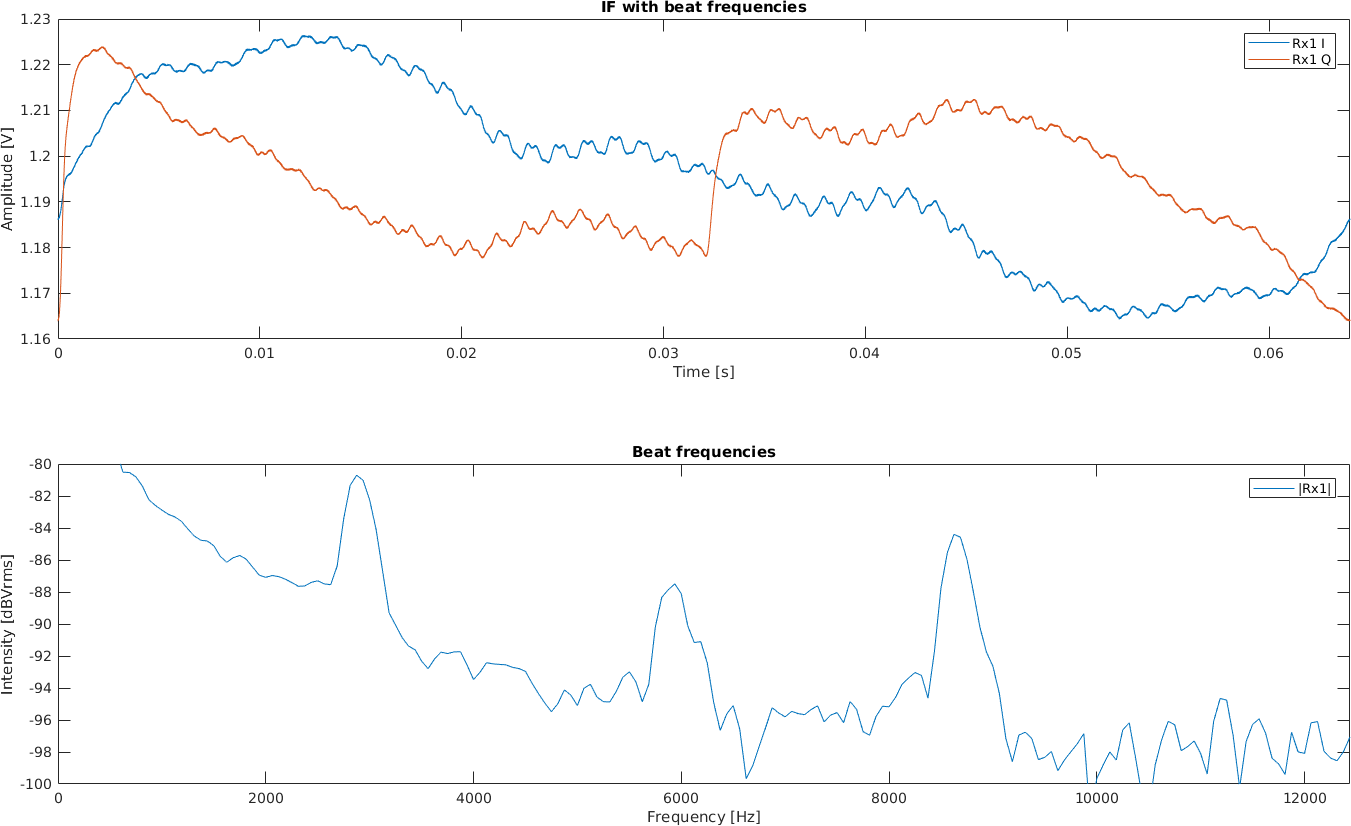
\includegraphics[max height=10cm,max width=10cm]{figures/fig_raw_beat.png}
    \caption{Beat signal and spectrum / range profile in a real-world measurement.}
\end{figure}

\subsection{Direction of Arrival}\label{direction-of-arrival}

A radar sensor with two or more receiving antennas which are separated
by not more than half a wavelength can measure the Direction of arrival
(DOA) of one or multiple targets. Because the echo from a target has to
travel a slightly longer distance to antennas further away, a phase
difference between the different antenna signals is measurable.

In the case of a pair of receiving antennas, the direction of arrival
\(\theta\) can be estimated \cite{VanZeijl2014} as

\[\theta = sin^{-1}\left({\frac{\lambda~\Delta\Phi}{2\pi ~d}}\right)\]

with wavelength \(\lambda\), antenna separation \(d\) and phase
difference \(\Delta\Phi\). \(\Delta\Phi\) is the angle difference
\(\angle S_1 - \angle S_2\) of the complex analytic antenna signals
\(S = S_I + j~S_Q\).

\begin{figure}[htp]
    \centering
    \label{fig:doa}
    \def\svgwidth{\linewidth}
    \input{gfx/diagrams/doa.pdf_tex}
    \caption{Direction of Arrival \(\theta\) can be estimated from phase difference \(\Delta\Phi\)}
\end{figure}

TODO
\cite{Hacker2010} \cite{Cho2017}

\subsection{Frequencies}\label{frequencies}

Even though radar applications exist for many frequencies, only a few of
them are OK to use for radiolocation and in home robots. The
``Industrial, Scientific, Medical'' (ISM) bands allows the unlicensed
use of some frequencies for radiolocation, including center frequencies
of \(24.125 GHz\), \(61.25 GHz\), \(122.5 GHz\) and \(245 GHz\).
Applications must however accept harmful interference \cite{FCC2017}.

The \(77 GHz\) band is ``restricted to vehicle-mounted field disturbance
sensors used as vehicle radar systems.'' (FCC Part 15 §15.253(c)) - ETSI
defines it as ``Automatic Cruise Control `long-range radar' operating at
\(77 GHz\). This enables a vehicle to maintain a cruising distance from
a vehicle in front.'' (EN 301 091). The German Bundesnetzagentur also
declares it ``Kraftfahrzeug-Kurzstreckenradar'' (Vfg 66 / 2014).

A \(24 GHz\) center frequency is a safe bet. There are many radar
systems available and it being an ISM band makes licensing much easier.
The drawback is the very limited maximum bandwidth of \(250MHz\) in this
band.

Some newer radars use the \(60 GHz\) ISM band. It allows a rather wide
bandwidth of up to \(9GHz\) in some regions (see figure \ref{fig:wigig} ).
According to equation \#REF, this gives a very good range resolution in
the order of few \(cm\). At these high frequencies, RF energy
attenuation in material increases noticably \cite{FerrisJr.1998}. The
effect is that \(60GHz\) waves are limited to short ranges of a few
\(m\) and don't usually penetrate walls.

\begin{figure}[htp]
    \centering
    \label{fig:attenuation}
    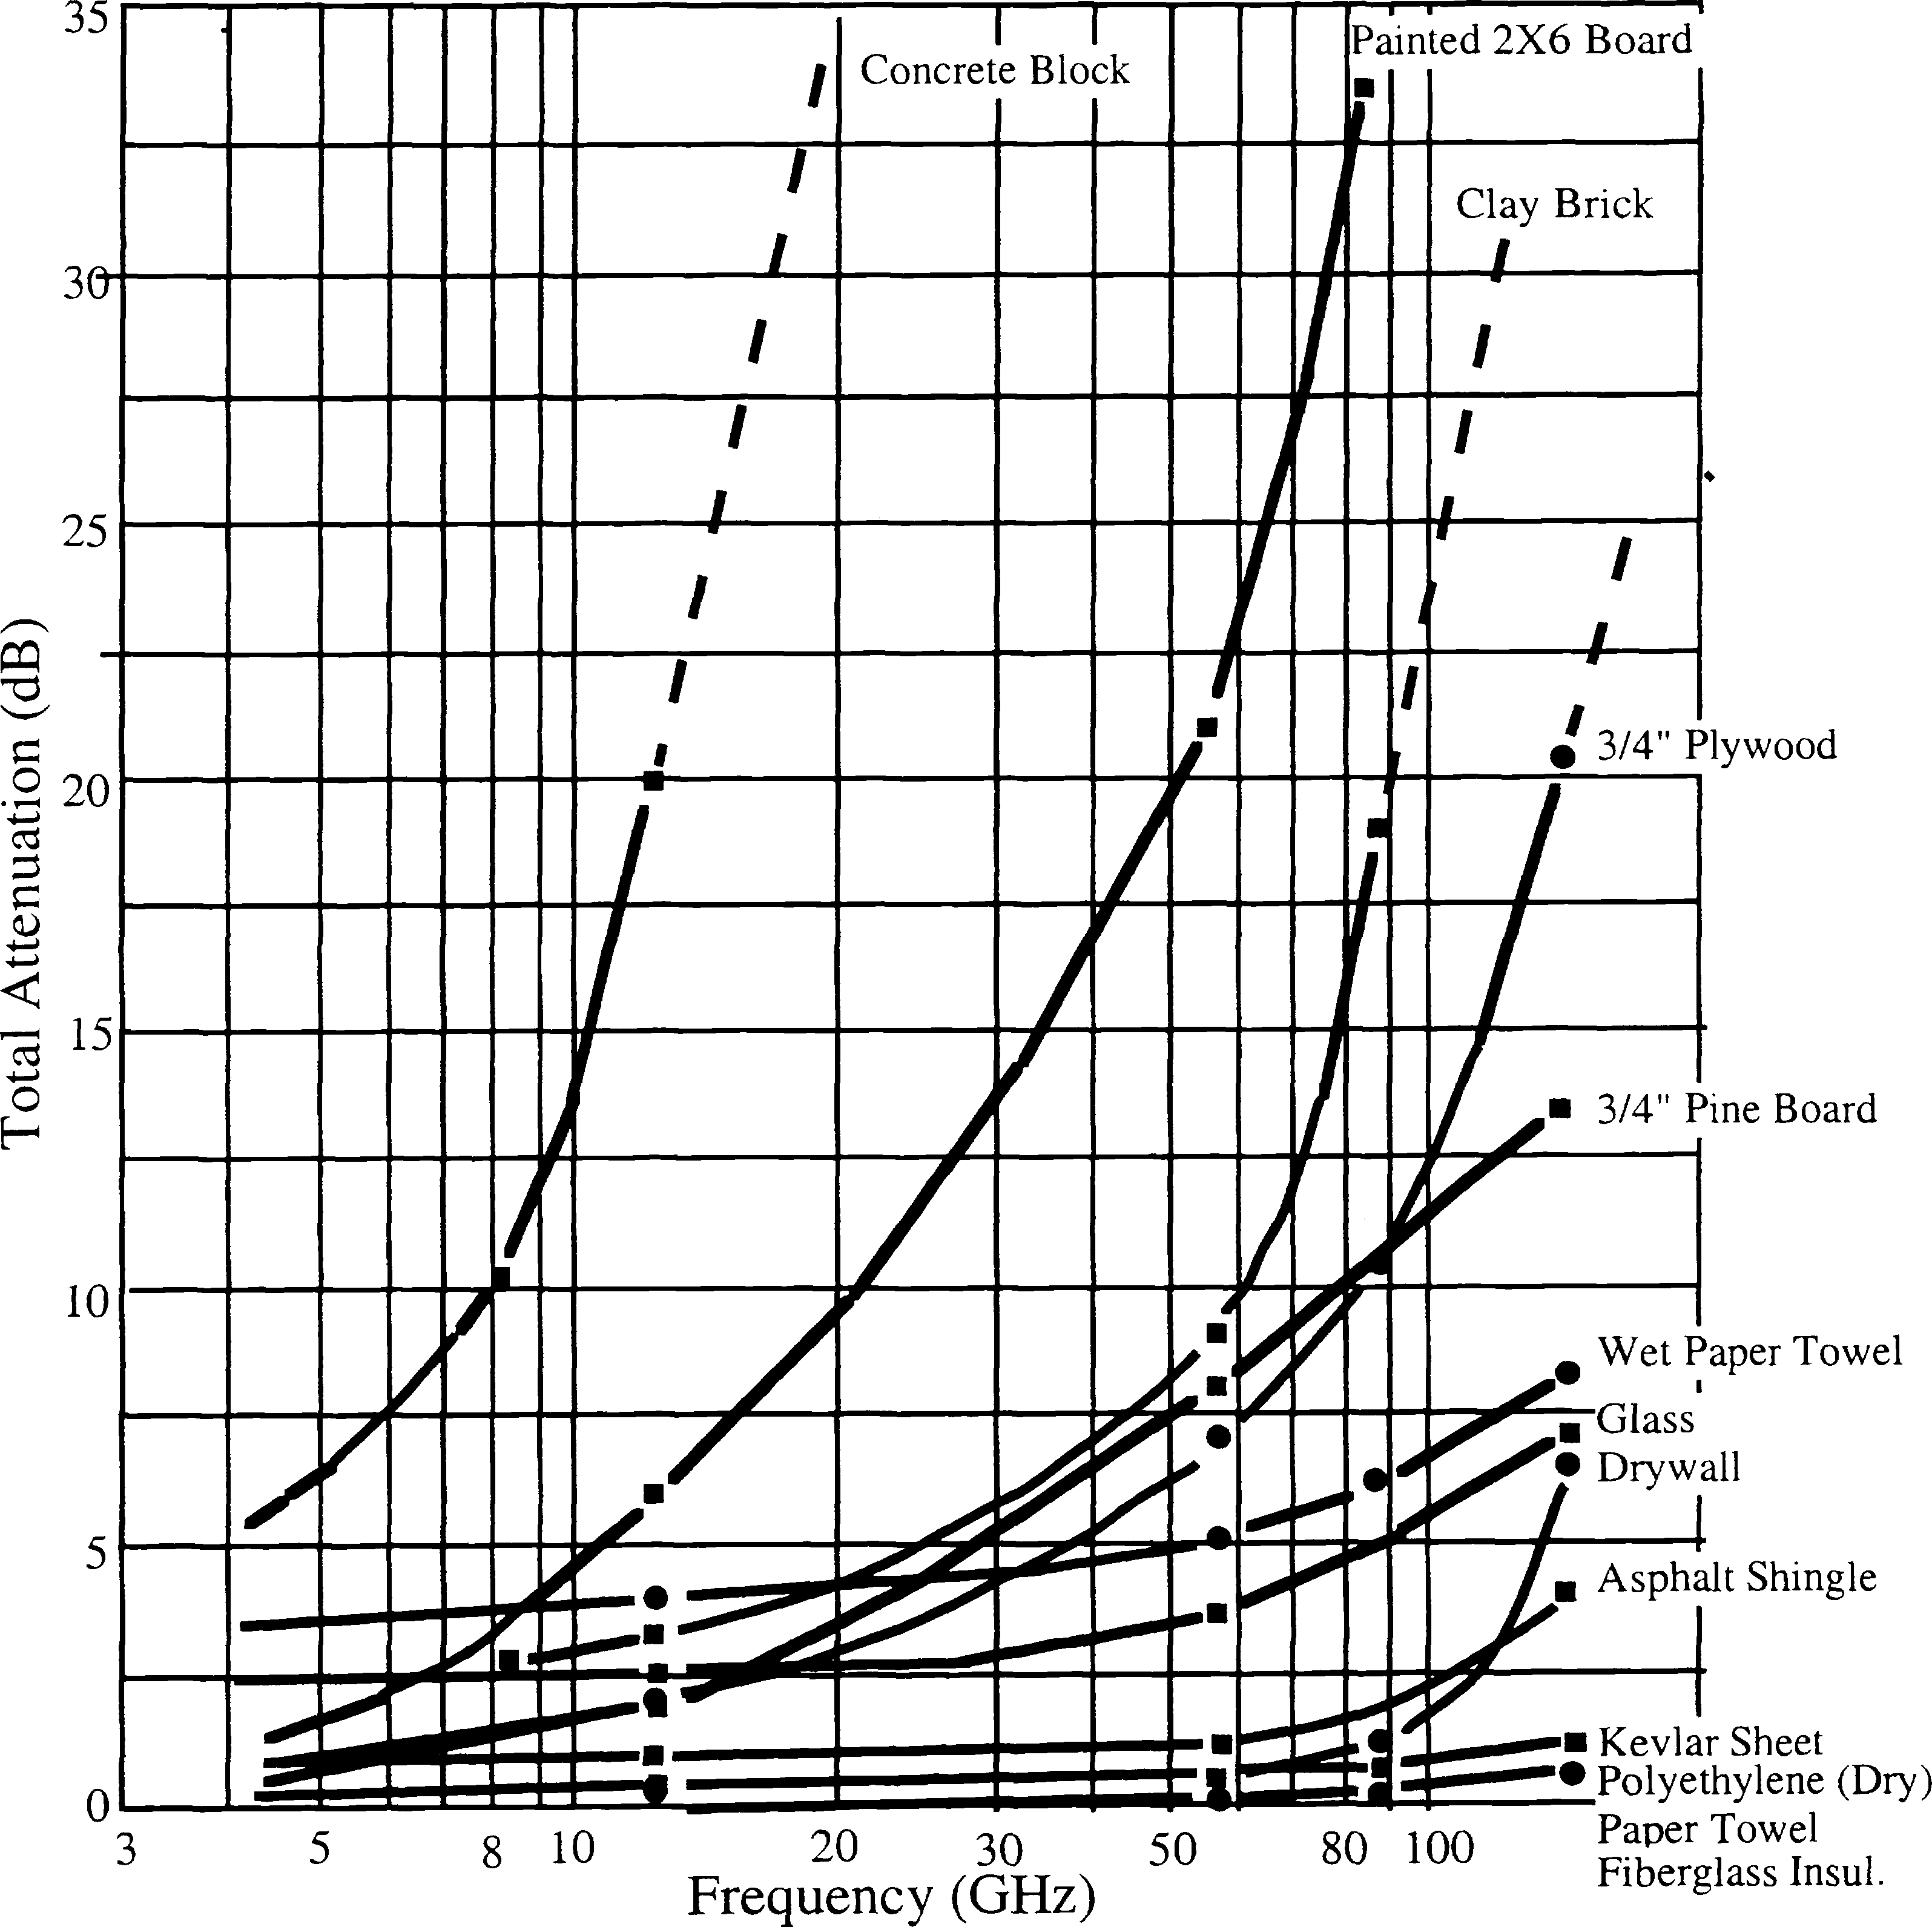
\includegraphics[max height=10cm,max width=10cm]{figures/rf_attenuation}
    \caption{Totl attenuation of RF energy when transmitted through various materials as a function of frequency. Source: \cite{FerrisJr.1998}}
\end{figure}

Atmospheric attenuation also limits long-range applications. In short
range (a few \(m\)) it should however not present a problem.

\begin{figure}[htp]
    \centering
    \label{fig:attenuation_air}
    
\includegraphics[max height=10cm,max width=10cm]{figures/ITU_0676-05}
    \caption{Specific RF attenuation due to atmospheric gases. Source: \cite{ITU1997}}
\end{figure}

The downside is that there are some other technologies using the same
frequency bands, most notably 802.11ad a.k.a.
WiGig\cite{AgilentTechnologies2013}. The WiGig frequency allocations in
figure \ref{fig:wigig} show in which regions the \(60GHz\) band is available (also
for radar).

\begin{figure}[htp]
    \centering
    \label{fig:wigig}
    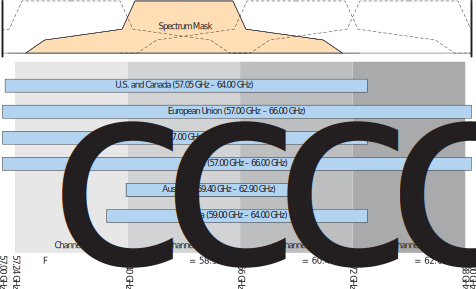
\includegraphics[max height=10cm,max width=10cm]{diagrams/spectrum}
    \caption{WiGig Channel Plan and Frequency Allocations by Region. Source: \cite{AgilentTechnologies2013}}
\end{figure}

\section{Overview of Radar
Research}\label{overview-of-radar-research}

Radar is used and researched since the 1940s. While it was historically
only used to detect aircraft and ships, it is an active research domain
in many fields today. Identification and localization of vessels is of
course still an important application in both civil and military
sectors. There is a great amount of research going into synthetic
aperture radar, in terrestrial imaging, but also general and concealed
imaging. Another area of research is radar antenna technology and
quasi-optics, which aims to find design improvements and more adapted
antennas for the manifold applications. Radar is used in human presence
detection and monitoring, including heartbeat detection. A new and very
promising discipline is radar-based gesture recognition, which enables
innovative human machine interaction applications. Indoor communication
and localization with radar beacons is another interesting and upcoming
technology. The radar-related research area that is most relevant for
mobile robots is radar-based slam.

\section{Existing radar-based solutions for map
building}\label{existing-radar-based-solutions-for-map-building}

\subsection{SAR}\label{sar}

In 1950 Doppler frequency analysis was found to improve image resolution
of side-looking radar, which led to the development of the synthetic
aperture radar (SAR) technique. SAR uses azimuth (along-track) motion to
synthesize an aperture that is longer than the physical size of the
radar antenna \cite{Wang2008}. The three major configurations are
stripmap SAR, scan SAR, and spotlight SAR. Current SAR systems can
operate in either mode by dividing their planar antenna into
sub-apertures, whose phase and amplitude are controlled by the
individual few hundred transmit/receive modules \cite{Moreira2013}.

\begin{figure}[htp]
    \centering
    \label{fig:sarmodes}
    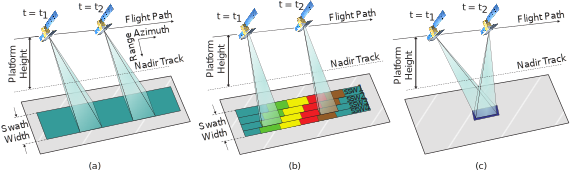
\includegraphics[max height=10cm,max width=10cm]{diagrams/sar}
    \caption{Illustration of different SAR operation modes which are used to increase the swath width (ScanSAR) or improve azimuth resolution (Spotlight) compared to Stripmap mode.
    (a) Stripmap. (b) ScanSAR. (c) Spotlight. Source: \cite{Moreira2013}}
\end{figure}

Radar echo data is sampled in both fast-time and slow-time, with
fast-time meaning the range scan dimension (fast, because the EM waves
travel at very high speed, \(c\)) and slow time denoting the azimuth or
along-track dimension (slow, because movement velocity will be
\(\ll c\)). This raw data does not give any useful information and needs
to be signal-processed first. Because SAR systems typically use
pulse-compressed radars, each range line needs to be convoluted with the
complex conjugate of the transmitted chirp's spectrum to obtain the
range-compressed
data\footnote{For the FMCW system used in the later parts of this thesis this is not necessary - the FMCW beat frequency spectrum is equivalent to the range-compressed data}.
In a second step, azimuth compression takes place by convolving the
signal in slow-time with the complex conjugate of the expected
azimuth-response from a target.

\begin{figure}[htp]
    \centering
    \label{fig:sarsteps}
    \includegraphics[max height=10cm,max width=10cm]{diagrams/sar2}
    \caption{Summary of SAR processing steps where the range compressed data result from a convolution of the raw data with the range reference function. In a second step the azimuth compression is performed through a convolution with the azimuth reference function, which changes from near to far range. Source: \cite{Moreira2013}}
\end{figure}

An elemental scatterer at range \(R(t)\) will return an echo \(s_a(t)\)
over time \(t\): \[
s_a(t) = P_r \sqrt{\sigma\vphantom{1}} \exp(j\varphi_s)\exp(j \underbrace{\frac{-4\pi}{\lambda}R(t)}_\text{az. phase var. $\omega_D$})
\] where \(P_r\) is the echo power of the received target, accounting
for dependencies like transmit power and path loss, \(\sigma\) is the
target's RCS, imaginary unit \(j\), \(\varphi_s\) the scattering phase,
and \(\frac{4\pi}{\lambda}R(t)\) the azimuth phase variation due to
changing distance \cite{Cumming2004}. The target's range \(R(t)\) is
described by the range at closest approach \(R_0\) and the radar's
(constant) movement speed \(v_R\): \[
R(t) = \sqrt{R_0^2+\left(v_Rt\right)^2} \approx R_0 + \frac{(v_Rt)^2}{2R_0} ~\text{for}~ \frac{v_Rt}{R_0} \ll 1
\] Substituting \#REF into the azimuth phase in \#REF and derivating
with respect to time yields the azimuth frequency \(f_D\) \[
\begin{aligned}
f_D &= \underbrace{\frac{1}{2\pi}}_{\omega_D = 2\pi f_D} \frac{\partial}{\partial t} \frac{-4\pi}{\lambda}  \underbrace{\left( R_0 + \frac{(v_Rt)^2}{2R_0}  \right)}_{R(t)} \\
&= -\frac{2v_R^2}{\lambda R_0}t
\end{aligned}
\] The azimuth frequency varies linearly with time \(t\) and is
inversely proportional to the closest approach (slant range) \(R_0\),
hence the azimuth reference function depends on geometry and is adapted
to range. Because of the frequency-shifting effect it is analogous to
and also called the Doppler frequency.

The most challenging aspect of SAR is the correction of range cell
migration induced defocusing. Range cell migration is visible in figure
\ref{fig:sarsteps}'s curvature of range compressed data. It occurs when a point
target's echo energy is distributed over several range cells, causing
azimuth defocusing. This effect is range-variant, as the curvature
depends on \(R_0\). Hence a non-stationary two-dimensional reference
function is necessary. There are several approaches in tackling this,
including the omega-k / wavenumber processor, range-Doppler, and chirp
scaling algorithms \cite{Moreira2013}.

\subsection{Scanning radar}\label{scanning-radar}

TODO

Small ground robots

\begin{itemize}
\item
  Martin Adams
\item
  Henrik Forsten
\item
  Gregory Charvat
\item
  Bat type radar
\end{itemize}

\subsection{Radar slam}\label{radar-slam}

TODO

Radar Slam

\begin{itemize}
\item
  Martin Adams
\item
  K2Pi
\end{itemize}
